% \AtBeginSection{
%   \begin{frame}{Sommaire}
%     \begin{columns}
%         \begin{column}{.6\textwidth}
%             \tableofcontents[currentsection]
%         \end{column}
%         \begin{column}{.4\textwidth}
%             \tikzstyle{flow-node} = [text centered, minimum height=2em, minimum width=5em, text width=5em, draw]
%             \tikzstyle{flow-start} = [rectangle, rounded corners, flow-node]
%             \tikzstyle{flow-process} = [rectangle, text centered, minimum height=2em, text width=10em, draw]
%             \tikzstyle{flow-data} = [trapezium, trapezium left angle=70, trapezium right angle=110, flow-node]
%             \tikzstyle{flow-decision} = [diamond, aspect=2.5, flow-node]
%             \tikzstyle{flow-arrow} = [thick, ->, >=latex, rounded corners]

%             \begin{adjustbox}{max width=\linewidth,max height=.95\textheight,valign=c}
%                 \begin{tikzpicture}[node distance=2em and 3em]
%                     \node (start) [flow-start] {Debut};
%                     \node (tal) [flow-data, below=of start] {Textes analysés};
%                     \node (enriched) [flow-process, below=of tal] {Enrichissement des arbres};
%                     \node (grammar) [flow-process, below=of enriched] {Extraction de la grammaire $G_i$};
%                     \node (check) [flow-decision, below=of grammar] {$G_i = G_T$};
%                     \node (end) [flow-start, left=of check] {Fin};
%                     \node (equiv) [flow-process, below=of check] {Construction des classes d'équivalence};
%                     \node (rewrite) [flow-process, below=of equiv] {Réécriture des arbres};

%                     \draw [flow-arrow] (start) -- (tal);
%                     \draw [flow-arrow] (tal) -- (enriched);
%                     \draw [flow-arrow] (enriched) -- (grammar);
%                     \draw [flow-arrow] (grammar) -- (check);
%                     \draw [flow-arrow] (check) -- node[above] {Oui} (end);
%                     \draw [flow-arrow] (check) -- node[left] {Non} (equiv);
%                     \draw [flow-arrow] (equiv) -- (rewrite);
%                     \draw [flow-arrow] (rewrite) |- + (3, -1) |- (grammar);
%                 \end{tikzpicture}
%             \end{adjustbox}
%         \end{column}
%     \end{columns}
%   \end{frame}
% }

\section{Grammaire et schéma}

\begin{frame}{}
    \setbeamercolor{block body}{bg=blue, fg=white}
    \begin{block}{}
        \Large
        \centering
        \vspace{.5em}
        Structuration automatique de l'information
        \vspace{.5em}
    \end{block}
\end{frame}

\begin{frame}{Exemple}
    \centering

    \begin{displaycquote}[extrait de PubMed]{mandalDeepBlueDot2022}
        A female patient in the age group 55-60 years presented to us with blurring of vision in both eyes.
        On slit-lamp examination, numerous circular to oval fleck-like discrete blue opacities at the level of deep corneal stroma and Descemet's membrane was observed.
    \end{displaycquote}

    \pause

    %\vfill

    \Huge$\Downarrow$\normalsize

    %\vfill

    \begin{figure}[htb]
        \small
        \begin{adjustbox}{max width=\linewidth}
            \begin{tikzpicture}[node distance=5em]
                \node[labeled node] (eyes) {Anatomy \nodepart{two} name: \emph{both eyes}};
                \node[labeled node, above=of eyes] (sosy) {Symptom \nodepart{two} name: \emph{blurring of vision}};
                \node[labeled node, right=7.5em of sosy] (person) {Person \nodepart{two} name: \emph{unknown}\\age: \emph{55-60}};
                \node[labeled node, right=7.5em of person] (exam) {Examination \nodepart{two} name: \emph{slit-lamp}};
                \node[labeled node, right=7.5em of exam] (result) {Symptom \nodepart{two} name: \emph{numerous circular}\\~~~~~~~~~~~\emph{to oval fleck-like}};
                \node[labeled node, below=of exam] (stroma) {Anatomy \nodepart{two} name: \emph{corneal stroma}};
                \node[labeled node, below=of result] (membrane) {Anatomy \nodepart{two} name: \emph{descemet membrane}};

                \path [very thick, -Latex]
                (person) edge node[labeled edge, anchor=center] {HasSym} (sosy)
                (sosy) edge node[labeled edge, anchor=center] {ConcernsAnat} (eyes)
                (person) edge node[labeled edge, anchor=center] {PassExam} (exam)
                (exam) edge node[labeled edge, anchor=center] {GivesRes} (result)
                (result) edge node[labeled edge, anchor=center] {ConcernsAnat} (stroma)
                (result) edge node[labeled edge, anchor=center] {ConcernsAnat} (membrane);
            \end{tikzpicture}
        \end{adjustbox}
    \end{figure}
\end{frame}

\begin{frame}{}
    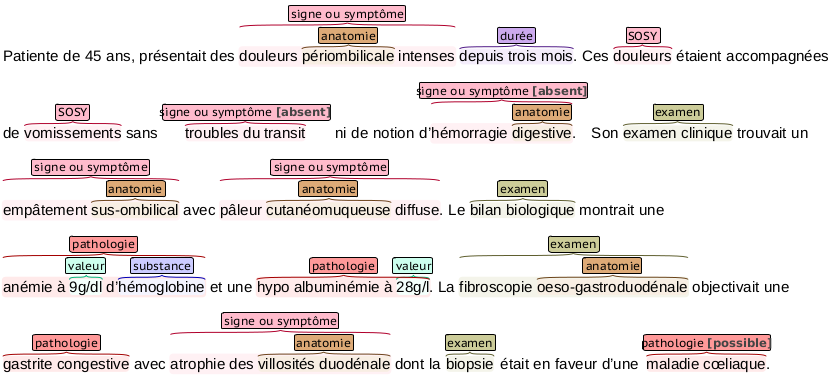
\includegraphics[width=\textwidth]{images/deft2020.png}
\end{frame}

\begin{frame}{Construction automatique de bases de données}
    \centering
    \begin{adjustbox}{max width=.8\linewidth}
        \begin{tabular}{cccccccc|l}
            Textes & $\rightarrow$ & $I_0$        & $\rightarrow$ & $ I_1$       & $\rightarrow$ & $ \dots$ & $I_t$        & Instances (arbres) \\
                   &               & $\downarrow$ &               & $\downarrow$ &               &          & $\downarrow$ &                    \\
                   &               & $G_0$        &               & $G_1$        &               & $ \dots$ & $G_t$        & Grammaires         \\
            %    &               & ~ $\searrow$  &               & $\downarrow$  &               &          & $\swarrow$ ~  &                    \\
            %    &               & \multicolumn{6}{c}{\fbox{Vérification par rapport à $\mathbb{G}$}}                       &
        \end{tabular}
    \end{adjustbox}

    \vfill

    \begin{block}{Objectif}
        % On cherche à réorganiser les informations contenues dans les textes (données non structurées) pour pouvoir les stocker dans une base de données.
        Réorganiser les informations non structurées des textes pour les stocker dans une base de données.
        L'approche se résume aux étapes suivantes :
        \begin{enumerate}
            \item Les entités nommées sont la base de l'information ;
            \item Les textes sont structurés selon une grammaire ;
            \item Réécrire l'instance pour obtenir une grammaire cible correspondant à un schéma de base de données ;
        \end{enumerate}
    \end{block}
\end{frame}

% \begin{frame}{Texte et arbres}
%     \begin{center}
%         \begin{adjustbox}{max width=\linewidth, max height=.5\textheight}
%             \begin{forest}
%                 where n children=0{tier=word}{}
%                 [S, for tree={s sep=2em}
%                     [NP
%                         [DT [la]]
%                         [NN,before computing xy={s/.average={s}{siblings}} [fréquence]]
%                         [NN [cardiaque]]
%                     ]
%                     [VP
%                         [VBD [était]]
%                         [PP
%                             [IN [à]]
%                             [NP
%                                 [CD [100]]
%                                 [NN [b/min]]
%                             ]
%                         ]
%                     ]
%                 ]
%             \end{forest}
%         \end{adjustbox}
%     \end{center}
% \end{frame}

\begin{frame}{Enrichissement}
    \begin{center}
        \begin{adjustbox}{max width=\linewidth, max height=.5\textheight}
            \only<1>{\begin{forest}
                    where n children=0{tier=word}{}
                    [S, for tree={s sep=2em}
                        [NP
                                [DT [la]]
                                [NN,before computing xy={s/.average={s}{siblings}} [fréquence]]
                                [NN [cardiaque]]
                        ]
                        [VP
                                [VBD [était]]
                                [PP
                                        [IN [à]]
                                        [NP
                                                [CD [100]]
                                                [NN [b/min]]
                                        ]
                                ]
                        ]
                    ]
                \end{forest}}
            \only<2>{\begin{forest}
                    where n children=0{tier=word}{}
                    [S, for tree={s sep=2em}
                        [NP
                                [DT [la]]
                                [{\color{blue}ENT\_EXAM}
                                    [NN [fréquence]]
                                    [NN [cardiaque]]
                                ]
                        ]
                        [VP
                                [VBD [était]]
                                [PP
                                        [IN [à]]
                                        [NP
                                                [CD [{\color{blue}ENT\_VALUE} [100]]]
                                                [NN [{\color{blue}ENT\_UNIT} [b/min]]]
                                        ]
                                ]
                        ]
                    ]
                \end{forest}}
            \only<3>{\begin{forest}
                    where n children=0{tier=word}{}
                    [S, for tree={s sep=2em}
                        [NP
                                [ENT\_EXAM
                                    [NN [fréquence]]
                                    [NN [cardiaque]]
                                ]
                        ]
                        [VP
                                [PP
                                        [NP
                                                [CD [ENT\_VALUE [100]]]
                                                [NN [ENT\_UNIT [b/min]]]
                                        ]
                                ]
                        ]
                    ]
                \end{forest}}
            \only<4>{\begin{forest}
                    where n children=0{tier=word}{}
                    [S, for tree={s sep=2em}
                        [ENT\_EXAM [fréquence] [cardiaque]]
                        [NP
                                [ENT\_VALUE [100]]
                                [ENT\_UNIT [b/min]]
                        ]
                    ]
                \end{forest}}
        \end{adjustbox}
        \vfill
        \only<2->{\begin{block}{Étapes}
                \begin{itemize}
                    %\item Unification des structures linguistique (conjonctions)
                    \only<2->{\item Insertion des entités dans l'arbre}
                    \only<3->{\item Supprimer termes et nœuds superflus}
                \end{itemize}
            \end{block}}
    \end{center}
\end{frame}

% \begin{frame}{Extraction de la grammaire (arbre quotient)}
%     \centering
%     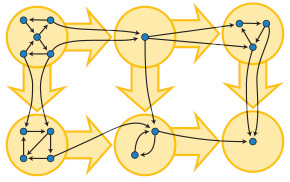
\includegraphics[height=.5\textheight]{images/Graph_Condensation.jpg}\\
%     {\tiny(Wikipédia 2024)}
% \end{frame}

\begin{frame}{Extraction de la grammaire (arbre quotient)}
    \begin{columns}
        \only<1>{\begin{column}{.5\textwidth}
                \centering
                \begin{forest}
                    for tree={circle,draw}
                    [, for tree={s sep=2em}
                        [
                            []
                                []
                        ]
                        [
                            []
                                [
                                    []
                                ]
                                [
                                    []
                                ]
                        ]
                    ]
                \end{forest}\\
                Arbre d'instance ($I_i$)
            \end{column}}%
        \only<2->{\begin{column}{.5\textwidth}
                \centering
                \begin{forest}
                    for tree={circle,draw}
                    [, fill=white, for tree={s sep=2em}
                        [, fill=red
                                [, fill=black]
                                [, fill=blue]
                        ]
                        [, fill=DarkGreen
                                [, fill=blue]
                                [, fill=red
                                        [, fill=black]
                                        % [, fill=blue]
                                ]
                                [, fill=red
                                        [, fill=black]
                                ]
                        ]
                    ]
                \end{forest}\\
                Arbre d'instance ($I_i$)
            \end{column}}%
        \only<3->{\begin{column}{.1\textwidth}
                \centering
                \LARGE
                $\Longrightarrow$
            \end{column}%
            \begin{column}{.4\textwidth}
                \centering
                \begin{forest}
                    for tree={circle,draw}
                    [, fill=white, for tree={s sep=2em}
                        [, fill=red
                                [, fill=black]
                                [, fill=blue]
                        ]
                        [, fill=DarkGreen
                                [, fill=blue]
                                [, fill=red
                                        [, fill=black]
                                        % [, fill=blue]
                                ]
                        ]
                    ]
                \end{forest}\\
                Arbre quotient ($S_i$)
            \end{column}}%
    \end{columns}
    \vspace{2em}
    \onslide<4->{\begin{block}{Grammaire ($G_i$)}
            \vspace{-1em}
            \begin{alignat*}{6}
                \drawCircle{white} & \to \drawCircle{red} ~ \drawCircle{DarkGreen} &  & \qquad\qquad \drawCircle{red} & \to \drawCircle{black} ~ \drawCircle{blue} &  & \qquad\qquad \drawCircle{DarkGreen} & \to \drawCircle{blue} ~ \drawCircle{red}^+
            \end{alignat*}
        \end{block}}
\end{frame}

% \begin{frame}{Extraction de la grammaire (arbre quotient)}
%     \begin{definition}[Grammaire quotient]
%         Étant donné un arbre $T$ et son quotient $Q_T = (Q_D, Q_l)$, la \gls{cfg} condensée $G_T = (N, T, P, \lambda)$ qui reconnaît $T$ est obtenue via $Q_T$ où :
%         \begin{itemize}
%             \item $\lambda$ est le symbole de départ ;
%             \item l'ensemble de non-terminaux $N$, éventuellement décorés par ${}^+$, est l'ensemble d'étiquettes $Q_l(u)$ pour toute position $u \in Q_D$ qui n'est pas une feuille ;
%             \item l'ensemble de terminaux $T$ est l'ensemble d'étiquettes $Q_l(u)$ pour toute position $u \in Q_D$ qui est une feuille ;
%             \item l'ensemble $P$ de règles de production contient, pour toute position $u \in Q_D$ qui n'est pas une feuille, les règles de la forme $Q_l(u) \to Q_l(u.0), \dots Q_l(u.i)$.
%         \end{itemize}
%     \end{definition}
% \end{frame}

% \begin{frame}{Extraction de la grammaire (arbre quotient)}
%     \begin{center}
%         \begin{adjustbox}{valign=c, max width=\textwidth, max height=.4\textheight}
%             \begin{forest}
%                 for tree={s sep=5em}
%                 [$\lambda$
%                 [$X$ [$a$] [$b$]]
%                     [$X$,before computing xy={s/.average={s}{siblings}} [$b$] [$c$]]
%                     [$Y$ [$a$]]
%                 ]
%             \end{forest}
%         \end{adjustbox}
%         \vfill
%         \pause
%         \begin{adjustbox}{valign=c, max width=\textwidth, max height=.4\textheight}
%             \begin{forest}
%                 for tree={s sep=20mm}
%                 [$\lambda$
%                 [$X^+$ [$a$] [$b$] [$c$]]
%                     [$Y$ [$a$]]
%                 ]
%             \end{forest}
%         \end{adjustbox}
%     \end{center}
% \end{frame}

%\section{Grammaire cible}

\begin{frame}{Grammaire cible}
    \begin{columns}
        \begin{column}{.6\textwidth}
            \only<-5>{\begin{description}
                    \uncover<2->{\item[Attribut] Une donnée associée à un nom}
                    \uncover<3->{\item[Groupe] Un ensemble nommé d'attributs distincts}
                    \uncover<4->{\item[Relation] Une relation entre deux groupes distincts}
                    \uncover<5->{\item[Collection] Un ensemble de groupes et de relations équivalents}
                \end{description}}
            \only<6->{\begin{alignat*}{2}
                    \lambda & \to COLL_1 ~ COLL_2 ~ COLL_3 \\
                    COLL_1  & \to GROUP_1^+                \\
                    COLL_2  & \to GROUP_2^+                \\
                    COLL_3  & \to REL_1^+                  \\
                    REL_1   & \to GROUP_1 ~ GROUP_2        \\
                    GROUP_1 & \to a ~ b                    \\
                    GROUP_2 & \to c                        \\
                    a       & \to \langle data \rangle     \\
                    b       & \to \langle data \rangle     \\
                    c       & \to \langle data \rangle
                \end{alignat*}}
        \end{column}
        \begin{column}{.4\textwidth}
            \begin{center}
                \begin{tikzpicture}[-latex,on grid]
                    \onslide<2->{\node (v1) at (0,0) {$v_1$};}
                    \onslide<2->{\node (v2) at (1.3,0) {$v_2$};}
                    \onslide<2->{\node (v3) at (2.6,0) {$v_3$};}
                    \onslide<2->{\node (a)  at (0,1.3) {a};}
                    \onslide<2->{\node (b)  at (1.3,1.3) {b};}
                    \onslide<2->{\node (c)  at (2.6,1.3) {c};}
                    \onslide<3->{\node (g1) at (0,2.6) {$GROUP_1$};}
                    \onslide<3->{\node (g2) at (2.6,2.6) {$GROUP_2$};}
                    \onslide<4->{\node (r)  at (1.3,3.9) {$REL_1$};}
                    \onslide<5->{\node (cr) at (1.3,5.2) {$COLL_{3}$};}
                    \onslide<5->{\node (c1) at (0,5.2) {$COLL_1$};}
                    \onslide<5->{\node (c2) at (2.6,5.2) {$COLL_2$};}

                    \only<2->{\path (a)  edge (v1);}
                    \only<2->{\path (b)  edge (v2);}
                    \only<2->{\path (c)  edge (v3);}
                    \only<3->{\path (g1) edge (a);}
                    \only<3->{\path (g1) edge (b);}
                    \only<3->{\path (g2) edge (c);}
                    \only<4->{\path (r)  edge (g1);}
                    \only<4->{\path (r)  edge (g2);}
                    \only<5->{\path (c1) edge (g1);}
                    \only<5->{\path (c2) edge (g2);}
                    \only<5->{\path (cr) edge (r);}
                \end{tikzpicture}
            \end{center}
        \end{column}
    \end{columns}
\end{frame}

\begin{frame}{Grammaire S-attribuée}
    \begin{example}
        \vspace{-1em}
        \begin{alignat*}{6}
            P_{\only<2->{val}} & \to 0 \quad &  & \onslide<3->{\color<4>{blue}[val \gets 0]} \qquad &  & P_{\only<2->{val}} & \to P_{\only<2->{val'}}~0 \quad & \onslide<3->{\color<5>{blue}[val \gets 2 * val']}       \\
            P_{\only<2->{val}} & \to 1 \quad &  & \onslide<3->{[val \gets 1]} \qquad                &  & P_{\only<2->{val}} & \to P_{\only<2->{val'}}~1 \quad & \onslide<3->{\color<6,7>{blue}[val \gets 2 * val' + 1]}
        \end{alignat*}
    \end{example}

    \vspace{1em}

    \begin{center}
        \small
        \begin{forest}
            where n children=0{tier=word}{}
            [{P \only<7->{($val=3$)}}, for tree={calign=last, s sep=2em}
                [{P \only<6->{($val=1$)}}
                        [{P \only<5->{($val=0$)}}
                                [{P \only<4->{($val=0$)}}
                                        [0]
                                ]
                                [0]
                        ]
                        [1]
                ]
                [1]
            ]
        \end{forest}
    \end{center}
\end{frame}

\begin{frame}{Méta-grammaire}
    \begin{definition}
        Une méta-grammaire $\mathbb{G} = (N, T, R, S)$ est une grammaire S-attribuée qui reconnaît l'ensemble de règles d'une CFG condensée.

        On distingue deux types de règles sémantiques pour une règle $r$ :
        \begin{itemize}
            \item $a \gets \alpha$ %où $a$ est l'attribut qui est évalué et $\alpha$
                  où $\alpha$ est une formule sur les attributs dans $r$ ;
            \item $\gamma \gets \beta$ où $\beta$ est une formule logique sur les attributs dans $r$.
                  \pause
                  \begin{itemize}
                      \item Si $S_\gamma = \top$, la dérivation est valide ;
                      \item Si $S_\gamma = \bot$, la dérivation est non valide.
                  \end{itemize}
        \end{itemize}
    \end{definition}
    %\vspace{-1em}
    \pause
    \small
    \begin{align*}
        \langle group_{name, eL} \rangle & ::= GROUP_{name} \to \langle entList_{eL} \rangle                                                    \\
        \langle entList_{eL} \rangle     & ::= ENT_{name}                                       & [eL \gets \{name\}]                           \\
                                         & ~~ \mid ~ ENT_{name} ~ \langle entList_{eL'} \rangle & [name \notin eL'; eL \gets \{name\} \cup eL']
    \end{align*}
\end{frame}

\begin{frame}{}
    \centering
    \begin{adjustbox}{max width=\linewidth,max height=.95\textheight,valign=c}
        \parbox{\linewidth}{\begin{align*}
                \epsilon                                    & ::= \langle root_{eL',gL',cgL',rL',crL'} \rangle ~\textsc{eol}~ \langle ruleList_{eL,gL,cgL,rL,crL} \rangle  & [eL' \subseteq eL; gL' \subseteq gL; cgL' \subseteq cgL; rL' \subseteq rL; crL' \subseteq crL]         \\
                \langle root_{eL,gL,cgL,rL,crL} \rangle     & ::= \lambda \to \langle rootList_{eL,gL,cgL,rL,crL} \rangle                                                                                                                                                           \\[1em]
                % Root list
                \langle rootList_{eL,gL,cgL,rL,crL} \rangle & ::= \epsilon                                                                                                 & [eL \gets \emptyset; gL \gets \emptyset; cgL \gets \emptyset; rL \gets \emptyset; crL \gets \emptyset] \\
                                                            & ~~ \mid ~ ENT_{name}  ~ \langle rootList_{eL',gL,cgL,rL,crL} \rangle                                         & [name \notin eL'; eL \gets \{name\} \cup eL']                                                          \\
                                                            & ~~ \mid ~ GROUP_{name} ~ \langle rootList_{eL,gL',cgL,rL,crL} \rangle                                        & [name \notin gL'; gL \gets \{name\} \cup gL']                                                          \\
                                                            & ~~ \mid ~ REL_{name}  ~ \langle rootList_{eL,gL,cgL,rL',crL} \rangle                                         & [name \notin rL'; rL \gets \{name\} \cup rL']                                                          \\
                                                            & ~~ \mid ~ COLL_{name} ~ \langle rootList_{eL,gL,cgL',rL,crL} \rangle                                         & [name \notin cgL'; cgL \gets \{name\} \cup cgL']                                                       \\
                                                            & ~~ \mid ~ COLL_{name} ~ \langle rootList_{eL,gL,cgL,rL,crL'} \rangle                                         & [name \notin crL'; crL \gets \{name\} \cup crL']                                                       \\[1em]
                % Rules list
                \langle ruleList_{eL,gL,cgL,rL,crL} \rangle & ::= \epsilon                                                                                                 & [eL \gets \emptyset; gL \gets \emptyset; cgL \gets \emptyset; rL \gets \emptyset; crL \gets \emptyset] \\
                                                            & ~~ \mid ~ \langle entity_{name}          \rangle ~\textsc{eol}~ \langle ruleList_{eL',gL,cgL,rL,crL} \rangle & [name \notin eL'; eL \gets \{name\} \cup eL']                                                          \\
                                                            & ~~ \mid ~ \langle group_{name, eL'}      \rangle ~\textsc{eol}~ \langle ruleList_{eL,gL',cgL,rL,crL} \rangle & [name \notin gL' \land eL' \subseteq eL; gL \gets \{name\} \cup gL']                                   \\
                                                            & ~~ \mid ~ \langle relation_{name, gL'}   \rangle ~\textsc{eol}~ \langle ruleList_{eL,gL,cgL,rL',crL} \rangle & [name \notin rL' \land gL' \subseteq gL; rL \gets \{name\} \cup rL']                                   \\
                                                            & ~~ \mid ~ \langle collGrp_{name,grpName} \rangle ~\textsc{eol}~ \langle ruleList_{eL,gL,cgL',rL,crL} \rangle & [name \notin cgL' \land grpName \in gL; cgL \gets \{name\} \cup cgL']                                  \\
                                                            & ~~ \mid ~ \langle collRel_{name,relName} \rangle ~\textsc{eol}~ \langle ruleList_{eL,gL,cgL,rL,crL'} \rangle & [name \notin crL' \land relName \in rL; crL \gets \{name\} \cup crL']                                  \\[1em]
                % Groups
                \langle group_{name, eL} \rangle            & ::= GROUP_{name} \to \langle entList_{eL} \rangle                                                                                                                                                                     \\
                \langle collGrp_{name,grpName} \rangle      & ::= COLL_{name} \to GROUP_{grpName}^+                                                                                                                                                                                 \\[1em]
                % Relations
                \langle relation_{name, gL} \rangle         & ::= REL_{name} \to GROUP_{name1} ~ GROUP_{name2}                                                             & [name1 \neq name2; gL \gets \{name1, name2\}]                                                          \\
                \langle collRel_{name,relName} \rangle      & ::= COLL_{name} \to REL_{relName}^+                                                                                                                                                                                   \\[1em]
                % Entities
                \langle entList_{eL} \rangle                & ::= ENT_{name}                                                                                               & [eL \gets \{name\}]                                                                                    \\
                                                            & ~~ \mid ~ ENT_{name} ~ \langle entList_{eL'} \rangle                                                         & [name \notin eL'; eL \gets \{name\} \cup eL']                                                          \\
                \langle entity_{name} \rangle               & ::= ENT_{name} \to \langle data \rangle \label{meta:entity}
            \end{align*}}
    \end{adjustbox}
\end{frame}

\section{Structuration automatique}

\begin{frame}{Structuration automatique}
    \centering

    \begin{adjustbox}{max width=\linewidth}
        \only<1>{\begin{tabular}{cccccccc|l}
                Textes & $\rightarrow$ & $I_0$                                                              & $\rightarrow$ & $ I_1$       & $\rightarrow$ & $ \dots$ & $I_t$        & Instances (arbres) \\
                       &               & $\downarrow$                                                       &               & $\downarrow$ &               &          & $\downarrow$ &                    \\
                       &               & $S_0$                                                              &               & $S_1$        &               & $ \dots$ & $S_t$        & Quotients          \\
                       &               & $\downarrow$                                                       &               & $\downarrow$ &               &          & $\downarrow$ &                    \\
                       &               & $G_0$                                                              &               & $G_1$        &               & $ \dots$ & $G_t$        & Grammaires         \\
                       &               & ~ $\searrow$                                                       &               & $\downarrow$ &               &          & $\swarrow$ ~ &                    \\
                       &               & \multicolumn{6}{c}{\fbox{Vérification par rapport à $\mathbb{G}$}} &
            \end{tabular}}
        \only<2>{\begin{tikzpicture}[node distance=1.5em and 2em]
                %\node (start) [flow-start] {Début};
                %\node (tal) [flow-data] {Textes analysés};
                \node (enriched) [flow-process] {Enrichissement des arbres};
                \node (grammar) [flow-process, right=of enriched] {Extraction de la grammaire $G_i$};
                \node (check) [flow-decision, right=of grammar] {$G_i = G_t$};
                \node (end) [flow-start, below=of check] {Fin};
                \node (equiv) [flow-process, right=of check] {Construction des classes d'équivalence};
                \node (rewrite) [flow-process, right=of equiv] {Réécriture des arbres};

                %\draw [flow-arrow] (start) -- (tal);
                %\draw [flow-arrow] (tal) -- (enriched);
                \draw [flow-arrow] (enriched) -- (grammar);
                \draw [flow-arrow] (grammar) -- (check);
                \draw [flow-arrow] (check) -- node[left] {Oui} (end);
                \draw [flow-arrow] (check) -- node[above] {Non} (equiv);
                \draw [flow-arrow] (equiv) -- (rewrite);
                \draw [flow-arrow] (rewrite) -| + (2, 1.5) -| (grammar);
            \end{tikzpicture}}
    \end{adjustbox}

    \vfill

    \begin{block}{Approche}
        \begin{itemize}
            \item Structuration par grammaires : des données textuelles à un schéma de base de données ;
            \item Itérations : unification d'éléments fréquents avec mesure de similarité ;
            \item Arrêt lorsque la structure n'est plus simplifiable.% (pouvant être enregistrée dans une base).
        \end{itemize}
    \end{block}
\end{frame}

% \begin{frame}
%     \begin{columns}
%         \begin{column}{.5\textwidth}
%             \begin{itemize}
%                 \item Processus itératif de structuration ;
%                 \vfill
%                 \item Unification par réécriture successive des structures équivalentes ;
%                 \vfill
%                 \item Arrêt lorsque la structure n'est plus simplifiable.
%             \end{itemize}
%         \end{column}
%         \begin{column}{.5\textwidth}


%             \begin{adjustbox}{max width=\linewidth,max height=.95\textheight,valign=c}

%             \end{adjustbox}
%         \end{column}
%     \end{columns}
% \end{frame}

\begin{frame}{Équivalence de sous-arbres}
    % Exemple d'arbres a unifier. Exemple de pas a pas du fonctionnement de l'equivalence
    \begin{itemize}
        \item Identifier les groupements similaires (ensemble d'entités)
        \item L'instance est incomplète, un groupe peut contenir qu'un sous-ensemble d'attributs
              \pause
        \item Équivalence régulière : \textquote{deux individus sont régulièrement équivalents s'ils sont connectés à des individus équivalents}
              \pause
        \item Utilisation de similarité contextuelle
    \end{itemize}

    \vfill

    \begin{equation*}
        sim_f(x, y) = \frac{\sum_{i=0}^{depth_{min}} \frac{1}{i + 1} \cdot f(P^x_i, P^y_i)}{\sum_{j=0}^{depth_{min}} \frac{1}{j + 1}} \label{eq:struct:sim}
    \end{equation*}
\end{frame}

\begin{frame}{Preuve de concept}
    \begin{block}{Objectif}
        Minimiser la taille de la grammaire
        \pause
        \begin{itemize}
            \item maximiser le support des groupes
            \item maximiser la taille des groupes
        \end{itemize}
    \end{block}

    \vfill
    \pause

    \begin{enumerate}
        \item Identifier les groupes candidats
        \item Extraire les sous-groupes fréquents
        \item Étendre les groupes avec d'autres informations\\(en maintenant sa classe d'équivalence)
        \item Identifier les collections de groupes ;
        \item Identifier les relations entre deux groupes ;
        \item Identifier les collections de relations.
    \end{enumerate}
\end{frame}

\begin{frame}{Exemple}
    \centering
    \begin{adjustbox}{max width=\linewidth}
        \begin{dependency}[theme=simple]
            \begin{deptext}[row sep=.2em, column sep=.1em]
                Il \& s'agit \& d'une \& femme \& de \& 32 ans \& enceinte \& de \& 14 semaines \\
                \& \& \& SEX \& \& AGE \& SOSY \& \& DURATION \\
            \end{deptext}
            \wordgroup{1}{4}{4}{sex}
            \wordgroup{1}{6}{6}{age}
            \wordgroup{1}{7}{7}{sosy}
            \wordgroup{1}{9}{9}{duration}
        \end{dependency}
    \end{adjustbox}

    \vfill

    \begin{adjustbox}{max width=\linewidth}
        \begin{dependency}[theme=simple]
            \begin{deptext}[row sep=.2em, column sep=.1em]
                L'homme \& est \& traité \& pour \& du \& diabètes \& depuis \& 5 ans \\
                SEX \& \& \& \& \& SOSY \& \& DURATION \\
            \end{deptext}
            \wordgroup{1}{1}{1}{sex}
            \wordgroup{1}{6}{6}{sosy}
            \wordgroup{1}{8}{8}{duration}
        \end{dependency}
    \end{adjustbox}
\end{frame}

\begin{frame}{Exemple}
    \centering
    \only<1>{\begin{adjustbox}{max width=\linewidth}
            \begin{forest}
                where n children=0{tier=word}{}
                [. [. [$ENT_{sex}$ [femme]] [$ENT_{age}$ [32 ans]]] [. [$ENT_{sosy}$ [enceinte]] [$ENT_{duration}$ [14 semaines]]]]
            \end{forest}\qquad
            \begin{forest}
                where n children=0{tier=word}{}
                [. [$ENT_{sex}$ [homme]] [$ENT_{sosy}$ [diabètes]] [$ENT_{duration}$ [5 ans]]]
            \end{forest}
        \end{adjustbox}}

    \only<2>{\begin{adjustbox}{max width=\linewidth}
            \begin{forest}
                where n children=0{tier=word}{}
                [. [$GROUP_{person}$ [$ENT_{sex}$ [femme]] [$ENT_{age}$ [32 ans]]] [$GROUP_{condition}$ [$ENT_{sosy}$ [enceinte]] [$ENT_{duration}$ [14 semaines]]]]
            \end{forest}\qquad
            \begin{forest}
                where n children=0{tier=word}{}
                [$GROUP_{profile}$ [$ENT_{sex}$ [homme]] [$ENT_{sosy}$ [diabètes]] [$ENT_{duration}$ [5 ans]]]
            \end{forest}
        \end{adjustbox}}

    \only<3>{\begin{adjustbox}{max width=\linewidth}
            \begin{forest}
                where n children=0{tier=word}{}
                [. [$GROUP_{person}$ [$ENT_{sex}$ [femme]] [$ENT_{age}$ [32 ans]]] [$GROUP_{condition}$ [$ENT_{sosy}$ [enceinte]] [$ENT_{duration}$ [14 semaines]]]]
            \end{forest}\qquad
            \begin{forest}
                where n children=0{tier=word}{}
                [. [$ENT_{sex}$ [homme]] [$GROUP_{condition}$ [$ENT_{sosy}$ [diabètes]] [$ENT_{duration}$ [5 ans]]]]
            \end{forest}
        \end{adjustbox}}

    \only<4>{\begin{adjustbox}{max width=\linewidth}
            \begin{forest}
                where n children=0{tier=word}{}
                [. [$GROUP_{person}$ [$ENT_{sex}$ [femme]] [$ENT_{age}$ [32 ans]]] [$GROUP_{condition}$ [$ENT_{sosy}$ [enceinte]] [$ENT_{duration}$ [14 semaines]]]]
            \end{forest}\qquad
            \begin{forest}
                where n children=0{tier=word}{}
                [. [$GROUP_{person}$ [$ENT_{sex}$ [homme]]] [$GROUP_{condition}$ [$ENT_{sosy}$ [diabètes]] [$ENT_{duration}$ [5 ans]]]]
            \end{forest}
        \end{adjustbox}}

    \only<5,6>{\begin{adjustbox}{max width=\linewidth}
            \begin{forest}
                where n children=0{tier=word}{}
                [$REL_{hasCondition}$ [$GROUP_{person}$ [$ENT_{sex}$ [femme]] [$ENT_{age}$ [32 ans]]] [$GROUP_{condition}$ [$ENT_{sosy}$ [enceinte]] [$ENT_{duration}$ [14 semaines]]]]
            \end{forest}\qquad
            \begin{forest}
                where n children=0{tier=word}{}
                [$REL_{hasCondition}$ [$GROUP_{person}$ [$ENT_{sex}$ [homme]]] [$GROUP_{condition}$ [$ENT_{sosy}$ [diabètes]] [$ENT_{duration}$ [5 ans]]]]
            \end{forest}
        \end{adjustbox}}

    \only<7>{\begin{adjustbox}{max width=\linewidth}
        \begin{tikzpicture}[node distance=15em]
            \node[labeled node] (Person) {Person \nodepart{two} sex: \emph{Femme}\\age: \emph{32}};
            \node[labeled node, right=of Person] (sosy) {Condition \nodepart{two} name: \emph{Enceinte}\\duration: \emph{14sem}};
            \node[labeled node, below=2em of Person] (Person2) {Person \nodepart{two} sex: \emph{Homme}};
            \node[labeled node, right=of Person2] (sosy2) {Condition \nodepart{two} name: \emph{diabètes}\\duration: \emph{5ans}};

            \path [very thick, -Latex]
            (Person)  edge node[labeled edge, anchor=center] {hasCondition} (sosy)
            (Person2) edge node[labeled edge, anchor=center] {hasCondition} (sosy2);
        \end{tikzpicture}
    \end{adjustbox}}

    \only<6->{\vfill
        \begin{block}{Grammaire}
            \vspace{-1em}
            \begin{adjustbox}{max width=\linewidth}
                \parbox{\linewidth}{\begin{alignat*}{4}
                    \lambda         & \to REL_{hasCondition}    & \qquad REL_{hasCondition} & \to GROUP_{person} ~ GROUP_{condition} \\
                    GROUP_{person}  & \to ENT_{sex} ~ ENT_{age} & \qquad GROUP_{condition}  & \to ENT_{sosy} ~ ENT_{duration}        \\
                    ENT_{sex}       & \to \langle data \rangle  & \qquad ENT_{age}          & \to \langle data \rangle               \\
                    ENT_{sosy}      & \to \langle data \rangle  & \qquad ENT_{duration}     & \to \langle data \rangle
                \end{alignat*}}
            \end{adjustbox}
        \end{block}
    }
\end{frame}

% \begin{frame}{Exemple}
%     \centering

%     \begin{block}{}
%         \begin{align*}
%             ROOT         & \to hasCondition       \\
%             hasCondition & \to Person ~ Condition \\
%             Person       & \to SEX ~ AGE          \\
%             Condition    & \to SOSY ~ DURATION
%         \end{align*}
%     \end{block} \pause

%     \vfill

%     \begin{adjustbox}{max width=.8\linewidth}
%         \begin{tikzpicture}[node distance=15em]
%             \node[labeled node] (Person) {Person \nodepart{two} sex: \emph{Femme}\\age: \emph{32}};
%             \node[labeled node, right=of Person] (sosy) {Condition \nodepart{two} name: \emph{Enceinte}\\duration: \emph{14sem}};
%             \node[labeled node, below=2em of Person] (Person2) {Person \nodepart{two} sex: \emph{Homme}};
%             \node[labeled node, right=of Person2] (sosy2) {Condition \nodepart{two} name: \emph{diabètes}\\duration: \emph{5ans}};

%             \path [very thick, -Latex]
%             (Person) edge node[labeled edge, anchor=center] {hasCondition} (sosy)
%             (Person2) edge node[labeled edge, anchor=center] {hasCondition} (sosy2);
%         \end{tikzpicture}
%     \end{adjustbox}
% \end{frame}

%\section{Conclusion}
\begin{frame}{Résultats}
    % \begin{itemize}
    %     \item Étude qualitative montrant des résultats prometteurs
    %           \begin{itemize}
    %               \item Regroupement sémantiquement correct
    %               \item On identifie des associations qui se recoupent
    %           \end{itemize}
    %     \item Défis liés à l'évaluation de la qualité des résultats
    % \end{itemize}

    \begin{adjustbox}{max width=.9\textwidth}
        \centering
        \parbox{\linewidth}{\begin{align*}
            GROUP_0                     \to & ~ ENT_{Dose} ~ ENT_{Frequence}  & \qquad GROUP_1                    \to & ~ ENT_{Examen} ~ ENT_{Valeur}   \\
                                            & ~ ENT_{Mode} ~ ENT_{Substance}  & \qquad GROUP_2                    \to & ~ ENT_{Frequence}               \\
                                            & ~ ENT_{Sosy} ~ ENT_{Traitement} & \qquad GROUP_4                    \to & ~ ENT_{Anatomie} ~ ENT_{Examen} \\
            GROUP_3                     \to & ~ ENT_{Dose} ~ ENT_{Examen}     & \qquad                                & ~ ENT_{Sosy}                    \\
                                            & ~ ENT_{Sosy} ~ ENT_{Substance}  & \qquad GROUP_6                    \to & ~ ENT_{Dose}                    \\
            GROUP_8                     \to & ~ ENT_{Examen} ~ ENT_{Sosy}     & \qquad GROUP_9                    \to & ~ ENT_{Mode}                    \\
            GROUP_{10}                  \to & ~ ENT_{Substance}               & \qquad GROUP_{11}                 \to & ~ ENT_{Anatomie}                \\
            REL_{10 \leftrightarrow 9}  \to & ~ GROUP_{10} ~ GROUP_9          & \qquad REL_{11 \leftrightarrow 8} \to & ~ GROUP_{11} ~ GROUP_8          \\
            REL_{2 \leftrightarrow 6}   \to & ~ GROUP_2 ~ GROUP_6
        \end{align*}}
    \end{adjustbox}

    \begin{block}{Travaux futurs}
        \begin{itemize}
            \item Évaluer différentes stratégies de réécriture
            \item Prendre en compte des valeurs : extraction de dépendances fonctionnelles \cite{papenbrockFunctionalDependencyDiscovery2015}
        \end{itemize}
    \end{block}
\end{frame}
